\chapter{Executive Overview} \label{ch:executvesum}


% \usepackage[table]{xcolor}
% \begin{center}
% \setlength{\fboxsep}{7pt}
% \setlength{\fboxrule}{0.4pt}
% \fcolorbox{black!35}{gray!5}{%
% \begin{minipage}{0.92\textwidth}
% \textbf{Selected Concept Snapshot}\\[0.4em]
% \textbf{Selected concept:} Concept A -- Booty Grasper\\
% \textbf{Platform:} Reusable tail-sitter VTOL UAV\\
% \textbf{Interaction:} Upward-launched net around the suspended payload\\
% \textbf{Recovery principle:} UAV weight and thrust guide the coupled system downward\\
% \textbf{Key strength:} Non-destructive capture with a single-UAV architecture\\
% \textbf{Main risk:} Net deployment and tethered-load control
% \end{minipage}%
% }
% \end{center}
% \begin{table}[htbp]
% \centering
% \scriptsize
% \renewcommand{\arraystretch}{1.3}
% \caption{Midterm Report Requirements Checklist}
% \label{tab:midterm_checklist}
% \begin{tabular}{|p{4.2cm}|p{6.5cm}|p{2.5cm}|c|}
% \hline
% \textbf{Component} & \textbf{Description} & \textbf{Responsible} & \textbf{Done} \\ \hline
% Work flow diagram & Adapt from project plan & Jan & $\square$ \\ \hline
% Work breakdown (WBS) & adapt from project plan. improve resolution & Jan & $\square$ \\ \hline
% Gantt Chart & improve and adapt. & Frederic & $\square$ \\ \hline
% Organogram & add roles for new phases & Piotr & \checkmark\\ \hline
% Risk map/assessment & Make it more technical and include stuff from actual conecpts. preliminary calculations & Tabara & $\checkmark$ \\ \hline
% DOT & plenty of DOTS for subsystems, this should prbly be per conceptual design?. & TBD & $\square$ \\ \hline
% Interface definition / N2 & define interfaces and system interaction & Jan& \checkmark \\ \hline
% Trade method \& rationale & Set up tradeoff and why?, from mission, airports & Frederic/Alex& \checkmark \\ \hline
% Trade criteria & Metrics used to evaluate design options. & &  \checkmark\\ \hline
% Criteria weight factors & Importance scaling for trade-off metrics. &Everbody, proofread: Alex &  \checkmark\\ \hline
% Trade summary table & Consolidated results of trade-off studies. & Fred/Alex&  \checkmark\\ \hline
% Ops \& logistics concept & Strategy for operation and maintenance. &PB GZ & $\square$ \\ \hline
% Sustainable development & Environmental impact and lifecycle strategy. &AM & $\square$ \\ \hline
% Sensitivity analysis & Evaluation of variable changes on design. &Frederic/Alex & \checkmark  \\ \hline
% Verification \& validation & Procedures for meeting requirements. & Piotr/Andrei &  \checkmark \\ \hline
% ROI / Operational profit & Financial analysis and profitability. & GIO &  \checkmark \\ \hline
% RAMS & Reliability, Availability, Maintainability, Safety. & PB GZ& $\square$ \\ \hline
% Performance analysis & Flight profile, take from concept design & AD AP & $\square$ \\ \hline
% Configuration \& layout & Internal and external General Arrangement. & all of us? & $\square$ \\ \hline
% Aircraft characteristics & Fuel, hydraulic, auxiliary, and power systems. & FR AT & $\square$ \\ \hline
% Aerodynamics & Analysis of lift, drag, and moments. & AM & $\square$ \\ \hline
% Structural characteristics & Loading, stress, bending, and flutter. & J idk & $\square$ \\ \hline
% Stability and control & Static/dynamic stability and effectiveness. & either AD or FR & $\square$ \\ \hline
% Material characteristics & Selected materials and mechanical properties. & J AM & $\square$ \\ \hline
% \end{tabular}
% \end{table}





% \subsection*{Mission Need and Objective}


BELLONA is an autonomous aerial system developed to safely locate, intercept, and recover uncooperative free-floating balloons. The project is motivated by the operational risk created when meteorological, scientific, commercial, or security-related balloons drift into controlled, restricted or populated airspace. In such cases, the main challenge is not only to reach the balloon, but to remove the hazard without creating a more dangerous situation through falling debris, uncontrolled descent or destructive countermeasures. \\

At this stage, the mission need is translated into a selected conceptual design. First, the key requirements and system drivers are defined, followed by structuring the design space through Design Option Trees, and developing five complete system concepts, and comparing them through a weighted trade-off. The selected architecture is Concept A, named \textit{Vertical Net Launch}: a reusable tail-sitter VTOL UAV that approaches the balloon-payload system from below, captures the suspended payload using a net launched upward, and then uses its weight and thrust to guide the coupled system toward a safe recovery zone. This concept is carried forward because it gives the strongest balance between safety, performance, reliability, and sustainability.


% FIGURE SUGGESTION:
% Add a compact mission concept figure here: detection/cueing -> launch -> intercept -> net capture -> controlled descent -> recovery.
% This should be a simple horizontal mission sequence diagram, not a detailed technical drawing.

% \begin{figure}[H]
% \centering
% \begin{tikzpicture}[
% node distance=0.9cm,
% box/.style={draw, rounded corners, align=center, minimum height=0.9cm, minimum width=2.3cm, font=\small},
% arrow/.style={->, thick}
% ]
% \node[box] (cue) {External\\cueing};
% \node[box, right=of cue] (launch) {Launch \&\\transit};
% \node[box, right=of launch] (track) {Terminal\\tracking};
% \node[box, right=of track] (capture) {Net\\capture};
% \node[box, right=of capture] (descent) {Controlled\\descent};
% \node[box, right=of descent] (recovery) {Recovery\\and reset};

% \draw[arrow] (cue) -- (launch);
% \draw[arrow] (launch) -- (track);
% \draw[arrow] (track) -- (capture);
% \draw[arrow] (capture) -- (descent);
% \draw[arrow] (descent) -- (recovery);
% \end{tikzpicture}
% \caption{Simplified BELLONA mission sequence for Concept A.}
% \label{fig:exec_mission_sequence}
% \end{figure}




\subsection*{Key Requirements and Design Drivers}

% The target is treated as an uncooperative balloon with no onboard control, no guaranteed communication link, and uncertain drift behaviour. The target envelope is a balloon diameter of 2-6 m, a possible payload mass up to 50 kg, and a payload-to-balloon tether length of up to 35 m. The selected system must be able to intercept the balloon up to an altitude of 6000 m and a horizontal ground range of 6000 m from the launch location. It must also remain feasible in sustained winds up to 13 m/s and gusts up to 21 m/s.\\



\begin{table}[H]
\centering
\small
\caption{Main design envelope used for the selected concept.}
\label{tab:exec_design_envelope}
\renewcommand{\arraystretch}{1.15}
\begin{tabularx}{0.95\textwidth}{@{}p{0.35\textwidth}X@{}}
\toprule
\textbf{Driver} & \textbf{Current design value / implication} \\
\midrule
Target balloon & Uncooperative, 2--6 m diameter \\
Payload & Up to 50 kg suspended payload \\
Interception envelope & Up to 6000 m altitude and 6000 m horizontal range \\
Wind condition & 13 m/s sustained wind, 21 m/s gusts \\
Interaction safety & Non-destructive, controlled descent, no uncontrolled debris \\
Recovery & Balloon, payload and deployed hardware should be recoverable where feasible \\
\bottomrule
\end{tabularx}
\end{table}
% The most important safety driver is that the interaction must be non-explosive, non-pyrotechnic, and controlled. The mission must avoid uncontrolled rupture, falling debris larger than 50 g. This immediately eliminates destructive concepts such as projectile puncture, propeller cutting, explosive separation or uncontrolled deflation. The system must also retain manual oversight, pre-flight go/no-go checks, and safe abort logic, since the mission takes place in or near civilian airspace.\\

%  The original acquisition-cost target is recognised as challenging for the expanded 6 km altitude and range envelope, so cost is treated as a critical design pressure rather than as a fully closed requirement.

% Electric-only energy storage, recoverability of the balloon and payload, minimal consumables, repairable modules, and end-of-life handling of batteries, electronics, composites, metals all influence the concept selection as well. 





\subsection*{Main Interfaces and Integration Drivers}
\label{subsec:concept_a_interfaces}


% The selected concept cannot be treated as a normal aircraft with an independent payload, because the balloon interaction mechanism becomes part of the aircraft load path after capture. The main system boundary includes the airborne UAS, propulsion system, aerodynamic surfaces, sensing suite, flight control system, power and electronics, communication link, structural airframe, balloon interaction mechanism, and ground segment. The target balloon, atmosphere, airspace infrastructure, recovery area, terrain, and surrounding public remain external elements, but they impose strong constraints on sensing, control, safety and recovery.

The most important integration driver is the mechanical interface between the balloon interaction subsystem and the structure. After net capture, loads pass from the payload into the net, tether, reel, hardpoint and then the central fuselage frame. This capture load path is more critical than many conventional flight loads because failure would directly lead to loss of control over the balloon-payload system. These parts must therefore be sized and verified as primary structural elements.   

A second integration driver is the coupling between propulsion, aerodynamics, and control. BELLONA must operate in vertical take-off, transition, wing-borne cruise, hover below the target, net launch, towing descent and final landing. The same propulsive system must provide hover authority, transition control, cruise efficiency and be able to maintain control after the tether is loaded. %Propeller placement, wing geometry, tail-sitter stability, centre-of-gravity location, and control allocation are therefore strongly coupled.

% A third integration driver is the sensing and control interface. The UAV must transition from externally cued navigation to onboard target acquisition and terminal relative navigation. The sensing system must provide enough accuracy for the aircraft to position itself below the payload before firing the net. This creates strict mounting, field-of-view, vibration, latency, power, and data-rate requirements for the sensor suite. Finally, the ground system remains a safety-critical interface, because it provides mission authorisation, recovery-zone coordination, manual override, abort decisions, and post-mission handling procedures.

% FIGURE SUGGESTION:
% Add a simplified N2/interface figure here.
% Do not use the full dense N2 chart from the main report unless it is readable.

\subsection*{Concept Generation and Trade-off Approach}




The concept generation process is structured around the main system-level choices required by the assignment: aerial platform, sensing and tracking approach, and balloon interaction strategy. The aerial platform determines range, altitude capability, hover control, energy demand, payload capacity, and operational cost. The sensing architecture determines how the system moves from coarse target cueing to terminal relative navigation. The interaction strategy determines whether the balloon-payload system can be captured, guided or deflated safely.

The retained design options were combined into five complete mission concepts. The concepts entering the trade-off are summarised in Table~\ref{tab:exec_concepts_summary}.

\begin{table}[H]
\centering
\small
\caption{Concepts carried into the Midterm trade-off.}
\label{tab:exec_concepts_summary}
\renewcommand{\arraystretch}{1.15}
\begin{tabularx}{\textwidth}{@{}p{0.10\textwidth}p{0.22\textwidth}X@{}}
\toprule
\textbf{ID} & \textbf{Concept} & \textbf{Core idea} \\
\midrule
A & Vertical Net Launch &
Single tail-sitter VTOL captures the suspended payload from below using an upward-launched net, then tows the coupled system down using UAV weight and thrust. \\

B & Pick and Drop &
Carrier eVTOL deploys several cooperative drones around the balloon-payload system, using net containment, controlled deflation, and guided parafoil descent. \\

C & Mechanical Clamping &
Lift-and-cruise eVTOL secures the payload or lower attachment using deployable clamping beams, then guides the system down with mass and thrust. \\

D & Cooperative Payload Net &
Three multirotors close a shared net around the payload or lower flight train and use the net's weight to overcome residual lift. \\

E & Kinetic Bolas &
Hybrid UAV launches a weighted bolas line around the suspension line and uses tether reel-out, UAV weight, and thrust to guide the target downward. \\
\bottomrule
\end{tabularx}
\end{table}




The concepts were compared using five main criteria: safety, reliability and complexity, intercept capability, sustainability and cost. 

\subsection*{Selected Concept}





Concept A achieved the highest weighted score. Concept E was the closest competitor, but its competitiveness relied mainly on its lower cost rather than on stronger technical performance. The sensitivity analysis showed that when cost was omitted, Concept A increased its lead over Concept E and remained first across the isolated engineering criteria. Concepts B and D were eliminated because their multi-vehicle architectures introduced high cost, high sequencing complexity, and several mission-critical transition points. Concept C remained technically credible but less robust than Concept A because of its mechanical clamping complexity and payload-geometry uncertainty.




\subsubsection{Propulsion, Performance and Aerodynamics}
\label{subsubsec:concept_a_prop_perf_aero}


The propulsion, performance and aerodynamics subsystem must support vertical take-off, transition, cruise, hover below the payload, towing descent, and landing. The tail-sitter layout is selected because it combines wing-borne cruise efficiency with hover capability during the capture phase, which a conventional fixed-wing aircraft cannot provide.

The main design challenges are transition control, thrust margin and stability while hovering and while carrying a tethered load. After capture, the balloon-payload system will introduce additional drag and pitch or yaw moments. The next design phase must therefore refine the propeller sizing, wing area, control surfaces, centre-of-gravity limits and performance margins for both free flight, hovering and post-capture descent.



% This subsystem is responsible for enabling the vertical take-off, transition, cruise climb, target approach, hover and alignment, net launch, towing descent and finally landing. The four-rotor tail-sitter layout is retained because it provides quadrotor-like hover control during the capture phase while allowing wing-borne flight during climb and transit. 

% The main aerodynamic challenge is transition reliability. The aircraft must move between vertical hover and horizontal flight without losing control authority, and this must remain possible when the payload. The final design phase must therefore refine the wing geometry, control surfaces, propeller sizing, centre-of-gravity limits, transition schedule, and thrust margins under both free-flight, hover and tethered-load cases.


\subsubsection{Sensing, Control and Electronics}
\label{subsubsec:concept_a_sce}





The sensing, control and electronics subsystem supports both normal flight and target-relative navigation. Basic stabilisation relies on IMU, GNSS and barometric data, while terminal approach requires onboard sensing to refine the externally provided balloon position. Candidate sensors include visual or infrared cameras, radar, and possibly short-range depth sensing for final alignment below the payload.

The main control challenge is that the UAV changes behaviour during the mission. Before capture, it flies as a tail-sitter; after capture, it becomes a tethered system connected to a drifting balloon-payload body. The controller must therefore handle target tracking, hover alignment, net launch, tether-load awareness, actuator margins, target-loss recovery, and abort modes. The electronics subsystem must provide reliable power distribution, protected wiring, thermal management, and communication with the ground segment.

\subsubsection{Structures, Materials and Sustainability}
\label{subsubsec:concept_a_structures_materials_sustainability}


% The structural concept is governed by two main load paths. The first is the conventional flight load path. The second is the capture load path, where the payload load passes through the net, tether, reel, hardpoint and central fuselage frame. The capture load path is the principal structural driver because failure at this interface would directly compromise mission safety. \\

%  CFRP/epoxy structures are preferred for wing skins and spars because of their high stiffness-to-mass ratio. Aluminium 6061-T6 is used as the baseline metal for moderate-load frames, brackets and landing supports, while aluminium 7075-T6, steel, and stainless steel are reserved for compact highly loaded fittings, shafts, inserts, motor mounts and tether hardpoints. Non-primary fairings and covers may use ASA printed parts, while EPDM rubber is suitable for replaceable contact and landing pads. The net, tether, and closure line use UHMWPE fibres because of their high strength-to-weight ratio and flexibility. \\

% Sustainability is integrated into the structural strategy by prioritising modularity, inspection, repairability, and material recovery. The aircraft is treated as a reusable platform with removable wing modules, accessible parts, replaceable soft goods. Composite primary parts are used only where their mass benefit justifies the more difficult end-of-life route. Metals are preferred at bolted and highly loaded local interfaces because they are easier to inspect, replace, and recycle. %The final design must define proof-load tests, damage inspection procedures, replacement limits for the net and tether, and end-of-life handling for batteries, electronics, composites, and metals.





The structure is driven by two main load paths: the normal flight load path and the capture load path. Flight loads pass through the wing, motor mounts, fuselage, battery bay, and landing supports, while capture loads pass through the net, tether, reel, hardpoint, and central fuselage frame. The capture load path is the main structural driver, since failure there would directly compromise payload restraint and mission safety. \\

A mixed-material strategy is used. CFRP/epoxy is preferred for mass-sensitive primary structures such as wing skins and spars. Aluminium 6061-T6 is used for general frames and brackets, while higher-strength metals such as aluminium 7075-T6, steel, or stainless steel are reserved for compact loaded fittings, motor mounts, pins, inserts, and tether hardpoints. ASA or PA-CF may be used for non-primary covers, EPDM for replaceable contact pads, and UHMWPE for the net, tether and closure lines. \\
 % sandwich panels???????????
This material choice supports a reusable and repairable design. The aircraft should have removable wing modules, accessible hardpoints, replaceable soft goods, and inspectable metallic fittings. In the next phase, the design must define proof-load tests, damage inspection procedures, replacement limits for the net and tether, and end-of-life handling for batteries, electronics, composites, and metals.

\subsubsection{Balloon Interaction Mechanism}
\label{subsubsec:concept_a_balloon_interaction}



The balloon interaction mechanism is based on capturing the suspended payload from below. The UAV hovers underneath the target and launches a 2.4 by 2.4 m trapezoidal pyramid-shaped net upward. Corner weights spread the net, while a closure line, tether, and reel system restrain the payload and allow the UAV to manage the load after capture. This is illustrated in \autoref{fig:paycap}.

\begin{figure}[H]
    \centering
    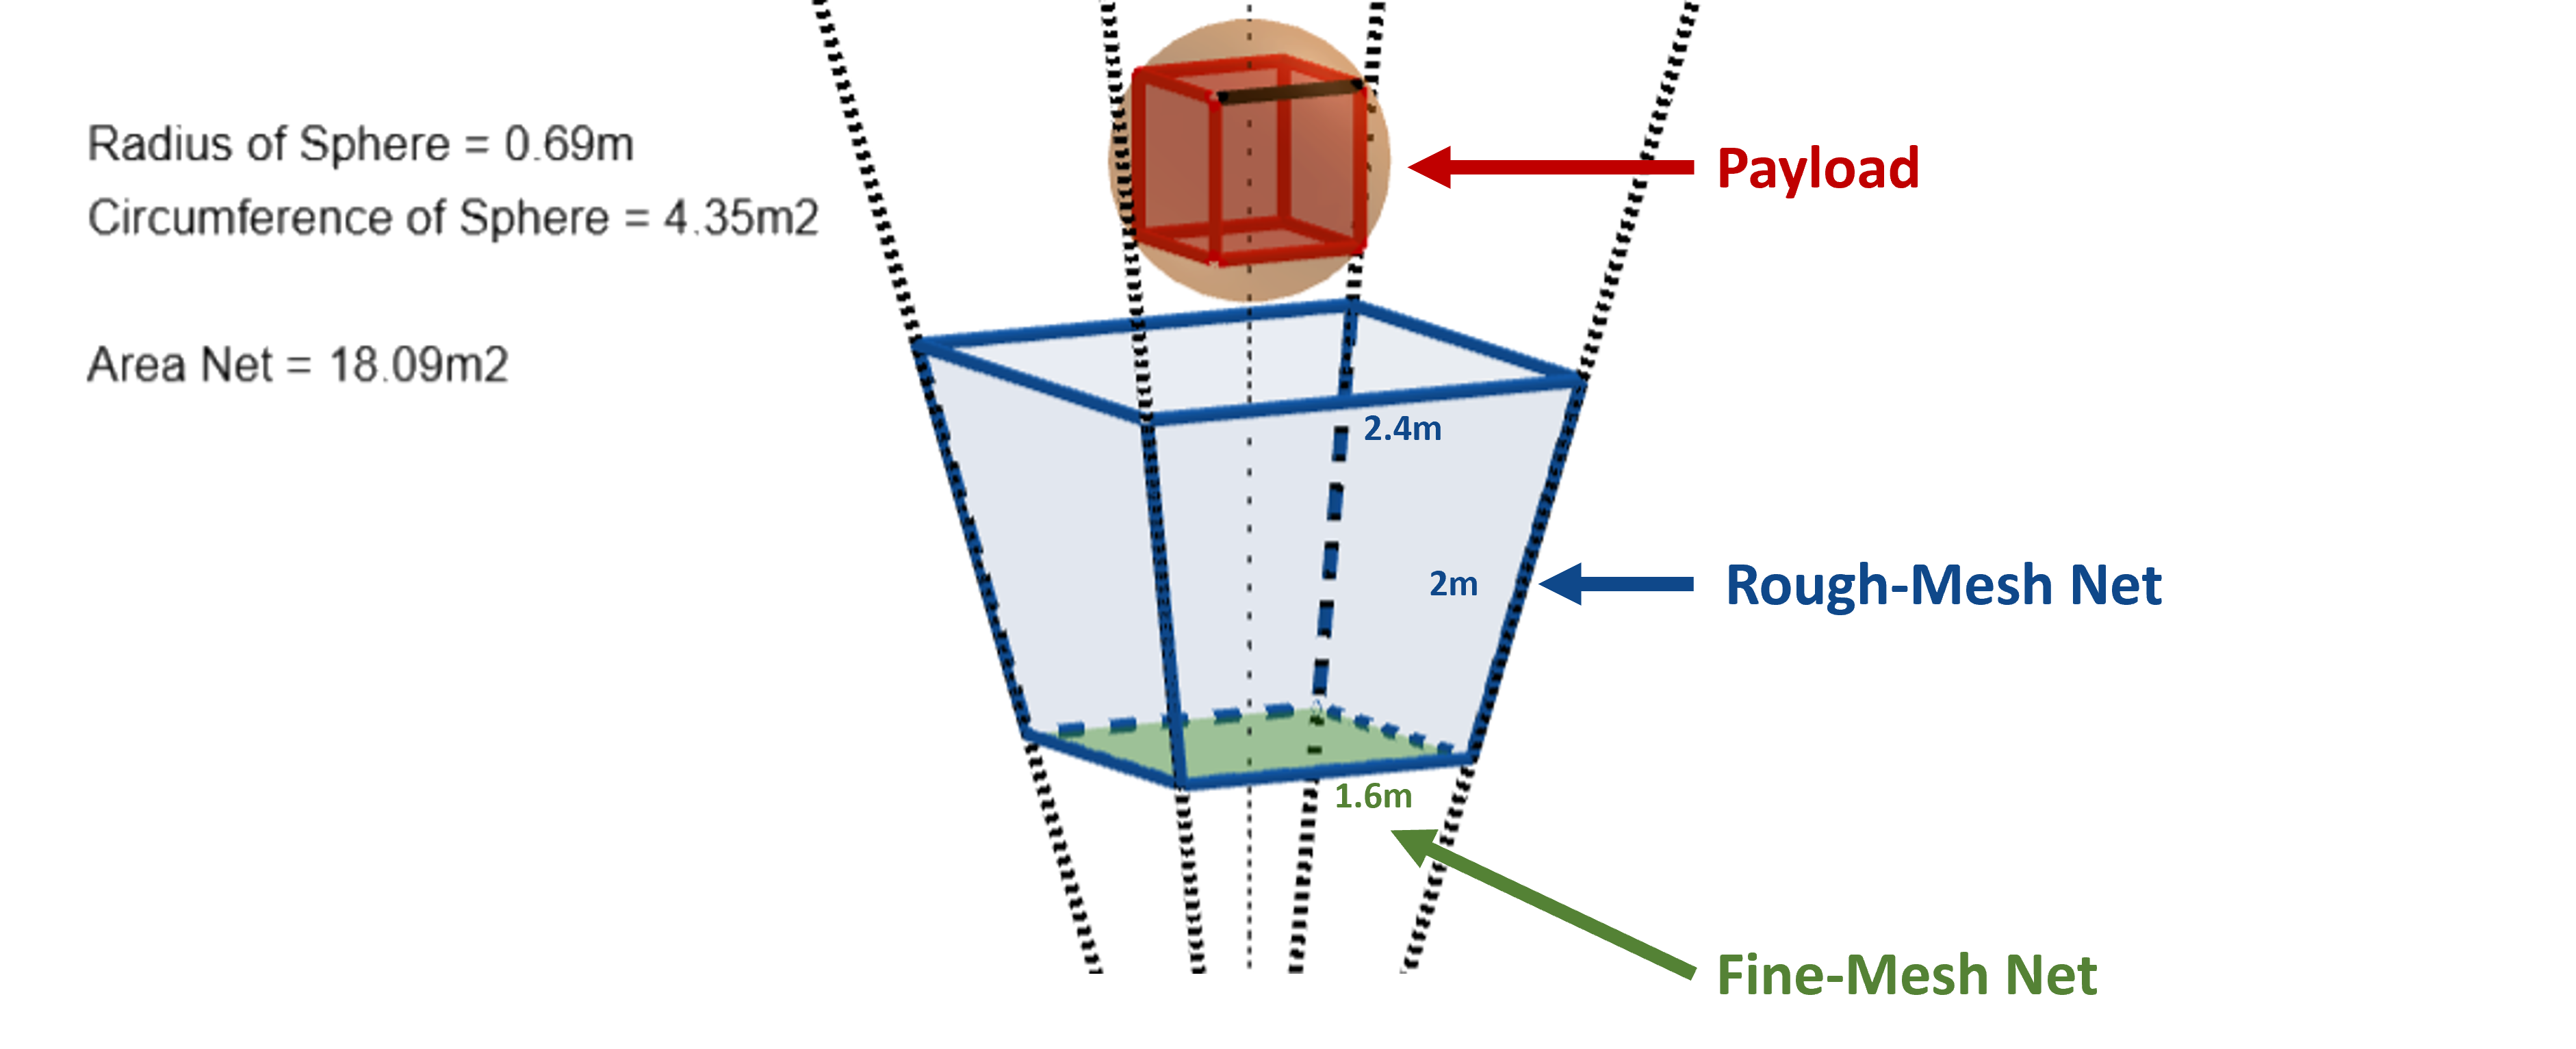
\includegraphics[width=0.7\linewidth]{figures/Payload Capture2.png}
    \caption{Sketch of the Payload Capture}
    \label{fig:paycap}
\end{figure}

This approach avoids intentional damage to the balloon envelope, reducing the risk of uncontrolled deflation and improving recoverability. The next design phase must size the net, corner weights, tether, reel torque, hardpoint loads and launch distance. It must also verify that failed or partial capture cannot pull the net into the propellers or block sensors.

An emergency breakaway system is required so that the UAV can disconnect if the balloon ruptures or the payload begins to fall uncontrollably. A small backup parachute attached to the UAV's end of the tether can then reduce the descent risk of the released payload-net system.

\subsubsection{Operations, Ground System and Safety}
\label{subsubsec:concept_a_operations_ground_safety}




The ground system supervises the mission from detection to recovery. Before launch, it checks the target cue, airspace, weather, battery state, system health and recovery-zone availability. During flight, it monitors telemetry, tracking status, link quality, energy margin, and interaction state.

The recovery zone may be updated during the mission based on wind drift, descent-start location, terrain, public exposure and crew accessibility. After landing, the recovery crew secures the UAV, payload, balloon material, net, tether, and any backup system. Safety is controlled through decision gates: pre-flight approval, target confirmation, safe interaction geometry, sufficient energy margin, acceptable recovery zone and abort availability.





% \begin{table}[H]
% \centering
% \small
% \caption{Executive subsystem summary for the selected Concept A architecture.}
% \label{tab:exec_subsystem_summary}
% \renewcommand{\arraystretch}{1.18}
% \begin{tabularx}{\textwidth}{@{}p{0.22\textwidth}X X@{}}
% \toprule
% \textbf{Subsystem area} & \textbf{Main role in Concept A} & \textbf{Main next-phase driver} \\
% \midrule

% Propulsion, performance and aerodynamics &
% Provide vertical take-off, transition, cruise, hover below the target, towing descent and landing capability. &
% Refine propeller sizing, wing area, transition control, thrust margin and stability with a tethered load. \\

% Sensing, control and electronics &
% Support normal flight, external cue handover, target-relative navigation, net-launch alignment and post-capture monitoring. &
% Define terminal sensor accuracy, sensor mounting, latency, power distribution, communication reliability and abort logic. \\

% Structures, materials and sustainability &
% Carry both conventional flight loads and the capture load path from payload to net, tether, reel, hardpoint and fuselage frame. &
% Size the primary hardpoint, reel support, central fuselage frame and inspectable/recyclable material interfaces. \\

% Balloon interaction mechanism &
% Capture the suspended payload using an upward-launched net, closure line, tether and reel without intentionally damaging the balloon envelope. &
% Verify net opening, partial-capture behaviour, tether tension, reel torque, emergency breakaway and propeller-clearance safety. \\

% Operations, ground system and safety &
% Supervise mission approval, target handover, recovery-zone updates, manual override, landing coordination and post-mission handling. &
% Define go/no-go gates, recovery-zone selection, telemetry monitoring, crew procedures and off-nominal mission responses. \\

% \bottomrule
% \end{tabularx}
% \end{table}


% The strongest coupling occurs between the balloon interaction mechanism, structure, propulsion and control system. Once the net is loaded, the UAV is no longer only an aircraft but part of a coupled balloon-payload-UAV system. The next design phase therefore focuses on closing the mass, power, control and structural margins around this post-capture condition.





\subsection*{Main Technical Risks and Verification Plan}

The main risks are concentrated in terminal approach, net deployment and post-capture descent. Critical failure cases include failed net opening, partial capture, net or tether interference with the UAV, loss of tracking, excessive payload swing and sudden loss of balloon lift.

Verification should therefore begin with analysis and simulation of capture loads, descent rates, tether dynamics, centre-of-gravity limits, propulsion margins, and recovery-zone footprints. Flight testing should progress from free tail-sitter flight to hover alignment, dummy net deployment, captive-load tests, and representative balloon-payload interaction tests.

\subsection*{Sustainability and Lifecycle Strategy}




The strongest sustainability benefit of Concept A is that it avoids intentional balloon destruction and aims to recover the balloon, payload, and interaction hardware without using unnecessary energy. The lifecycle strategy therefore focuses on reuse, repairability, battery health tracking. 


\begin{wrapfigure}{l}{0.60\textwidth}
    \centering
    \vspace{-0.5em}
    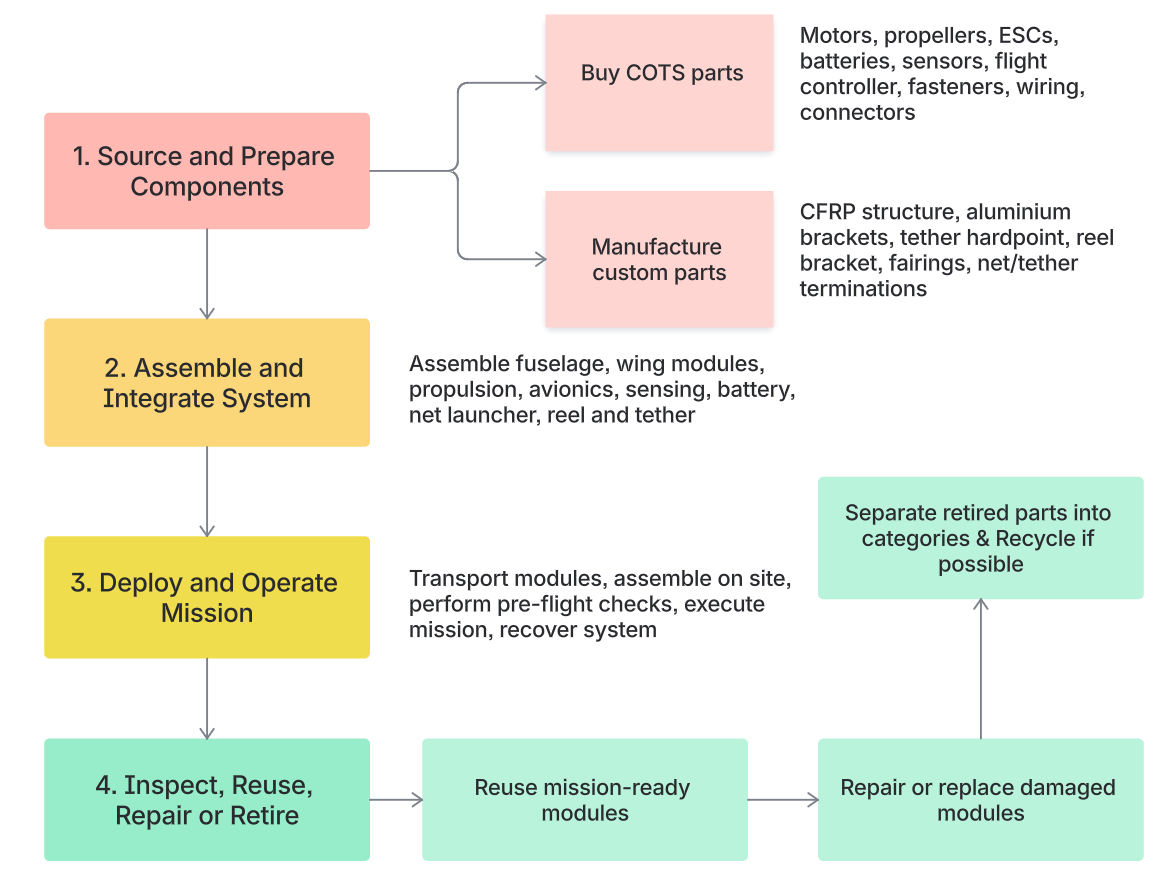
\includegraphics[width=0.60\textwidth]{figures/image.png}
    \caption{Simplified manufacturing, deployment, and life-cycle flow for Concept A.}
    \label{fig:exec_manufacturing_lifecycle_flow}
    \vspace{-1em}
\end{wrapfigure}



The material strategy supports this approach by using recyclable metals for inspectable fittings and hardpoints, CFRP only where mass savings are important, and UHMWPE/Dyneema for replaceable net and tether elements. In the next phase, a simple life-cycle inventory should be made for the main material groups, including metals, composites, polymers, batteries, electronics, and consumables, to show which parts are reusable, repairable, recyclable, or require controlled disposal. \\


\subsection*{Economic Outlook and Next Design Phase}




The economic model treats BELLONA as a reusable UAS sold to operators such as airports, border agencies, with additional revenue from maintenance and support. The current estimate gives a unit sales price of EUR 24,875, a production cost of EUR 17,100 per unit, and an operator mission cost of approximately EUR 150 per sortie. These values remain preliminary and must be refined once the propulsion, sensing, structural, and interaction subsystems are sized in more detail.

The next design phase should therefore focus on reducing uncertainty in the mass, cost, and manufacturing assumptions. The main priorities are to freeze the Concept A layout, refine the propulsion and battery sizing, size the capture load path, verify the net and tether mechanism, and update the financial model using supplier-based component prices.

























